% ---------------------------------------------------------------------------------------------------------------
% TEMPLATE PARA TRABALHO DE CONCLUSÃO DE CURSO
% Universidade Tecnológica Federal do Paraná - UTFPR
% Customização da classe abnTeX2 (http://www.abntex.net.br/) para as normas da UTFPR
%
% ADAPTADO DO Projeto hospedado em: <link git>
% Autores: Diego Marczal  <>
% 	   Michael Vornes <https://github.com/mvornes>
%
%----------------------------------------------------------------------------------------------------------------
% Codificação: UTF-8
% LaTeX:  abnTeX2          
% ---------------------------------------------------------------------------------------------------------------
\title{templateBSI}


% CARREGA CLASSE PERSONALIZADA DA UTFPR--------------------------------------------------------------------------
\documentclass[%twoside,                   % Impressão em frente e verso
    	        oneside,                   % Impressão apenas frente
]{configuracoes/utfpr-abntex2}


% INCLUI ARQUIVOS DE CONFIGURAÇÕES-------------------------------------------------------------------------------
% REFERÊNCIAS------------------------------------------------------------------
\usepackage[%
    alf,
    abnt-emphasize=bf,
    bibjustif,
    recuo=0cm,
    abnt-url-package=url,       % Utiliza o pacote url
    abnt-refinfo=yes,           % Utiliza o estilo bibliográfico abnt-refinfo
    abnt-etal-cite=3,
    abnt-etal-list=3,
    abnt-thesis-year=final
]{abntex2cite}                  % Configura as citações bibliográficas conforme a norma ABNT

% PACOTES----------------------------------------------------------------------
\usepackage[final]{pdfpages}
\usepackage{booktabs}                                       % Réguas horizontais em tabelas
\usepackage{color, colortbl}                                % Controle das cores
\usepackage{float}                                          % Necessário para tabelas/figuras em ambiente multi-colunas
\usepackage{graphicx}                                       % Inclusão de gráficos e figuras
\usepackage{icomma}                                         % Uso de vírgulas em expressões matemáticas
\usepackage{indentfirst}                                    % Indenta o primeiro parágrafo de cada seção
\usepackage{microtype}                                      % Melhora a justificação do documento
\usepackage{multirow, array}                                % Permite tabelas com múltiplas linhas e colunas
\usepackage{subeqnarray}                                    % Permite subnumeração de equações
\usepackage{lastpage}                                       % Para encontrar última página do documento
\usepackage{verbatim}                                       % Permite apresentar texto tal como escrito no documento, ainda que sejam comandos Latex
\usepackage{amsfonts, amssymb, amsmath}                     % Fontes e símbolos matemáticos
\usepackage[algoruled, portuguese]{algorithm2e}             % Permite escrever algoritmos em português
\usepackage[scaled]{helvet}                                % Usa a fonte Helvetica
%\usepackage{times}                                          % Usa a fonte Times
%\usepackage{palatino}                                      % Usa a fonte Palatino
%\usepackage{lmodern}                                       % Usa a fonte Latin Modern
\usepackage[bottom]{footmisc}                               % Mantém as notas de rodapé sempre na mesma posição
\usepackage{ae, aecompl}                                    % Fontes de alta qualidade
\usepackage{latexsym}                                       % Símbolos matemáticos
\usepackage{lscape}                                         % Permite páginas em modo "paisagem"
%\usepackage{picinpar}                                      % Dispor imagens em parágrafos
%\usepackage{scalefnt}                                      % Permite redimensionar tamanho da fonte
\usepackage{subfig}                                        % Posicionamento de figuras
%\usepackage{upgreek}                                       % Fonte letras gregas
%pra codigo python
\usepackage{listings}
\usepackage{pdfpages}
\usepackage{lipsum}
\usepackage[utf8]{inputenc}
\usepackage[brazil]{babel}
\usepackage[T1]{fontenc}
\usepackage{lmodern}



\lstset{language=C,
keywords={do, break,case,catch,continue,else,elseif,end,for,function,global,if,otherwise,persistent,return,switch,try,while,int, float, char},
basicstyle = \ttfamily, % \footnotesize, % Tamanho da fonte do código
numbers = left, % Posição da numeração das linhas
numberstyle = \tiny\color{blue}, % Estilo da numeração de linhas
stepnumber = 1, % Numeração das linhas ocorre a cada quantas linhas?
numbersep = 10pt, % Distância entre a numeração das linhas e o código
backgroundcolor = \color{white}, % Cor de fundo
showspaces = false, % Exibe espaços com um sublinhado
showstringspaces = false, % Sublinha espaços em Strings
showtabs = false, % Exibe tabulação com um sublinhado
%frame = single, % Envolve o código com uma moldura, pode ser single ou trBL
%rulecolor = \color{black}, % Cor da moldura
tabsize = 2, % Configura tabulação em x espaços
captionpos = b, % Posição do título pode ser t (top) ou b (bottom)
breaklines = true, % Configura quebra de linha automática
breakatwhitespace= false, % Configura quebra de linha
title = \lstname, % Exibe o nome do arquivo incluido
%caption = \lstname, % Também é possível usar caption no lugar de title
keywordstyle = \color{blue}, % Estilo das palavras chaves
commentstyle = \color{gray}, % Estilo dos Comentários
}

% Seleção de código de fonte
% Redefine a fonte para uma fonte similar a Arial (fonte Helvetica)
%\renewcommand*\familydefault{\sfdefault}

\usepackage[normalem]{ulem}


% CONFIGURAÇÕES DE APARÊNCIA DO PDF FINAL--------------------------------------
\makeatletter
\hypersetup{%
    portuguese,
    colorlinks=true,   % true: "links" coloridos; false: "links" em caixas de texto
    linkcolor=black,    % Define cor dos "links" internos
    citecolor=black,    % Define cor dos "links" para as referências bibliográficas
    filecolor=black,    % Define cor dos "links" para arquivos
    urlcolor=black,     % Define a cor dos "hiperlinks"
    breaklinks=true,
    pdftitle={\@title},
    pdfauthor={\@author},
    pdfkeywords={abnt, latex, abntex, abntex2}
}
\makeatother

% ALTERA O ASPECTO DA COR AZUL--------------------------------------------------
\definecolor{blue}{RGB}{41,5,195}

% REDEFINIÇÃO DE LABELS---------------------------------------------------------
\renewcommand{\algorithmautorefname}{Algoritmo}
\def\equationautorefname~#1\null{Equa\c c\~ao~(#1)\null}

\captionsetup{position=bottom}

% CRIA ÍNDICE REMISSIVO---------------------------------------------------------
\makeindex

% HIFENIZAÇÃO DE PALAVRAS QUE NÃO ESTÃO NO DICIONÁRIO---------------------------
\hyphenation{%
    qua-dros-cha-ve
    Kat-sa-gge-los
}



% INCLUI ARQUIVOS DO TRABALHO DE CONCLUSÃO DE CURSO (PRÉ-TEXTUAIS, TEXTUAIS, PÓS-TEXTUAIS)-----------------------

% INSERE CAPA E FOLHA DE ROSTO
% CAPA---------------------------------------------------------------------------------------------------

% ORIENTAÇÕES GERAIS-------------------------------------------------------------------------------------
% Caso algum dos campos não se aplique ao seu trabalho, como por exemplo,
% se não houve coorientador, apenas deixe vazio.
% Exemplos: 
% \coorientador{}
% \departamento{}

% DADOS DO TRABALHO--------------------------------------------------------------------------------------
\titulo{Colonialismo Digital e Resistência Popular: A Insurgência do Núcleo de Tecnologia do MTST}
%Termografia Dinâmica para Auxílio na detecção de indicadores de Câncer de Mama
\titleabstract{Digital Colonialism and Popular Resistance: The Insurgency of the MTST Technology Sector}
\autor{Melissa Fernanda Rodrigues Siqueira}
\autorcitacao{SIQUEIRA, Melissa; } % Sobrenome em maiúsculo
\local{Curitiba}
\data{2025}

% NATUREZA DO TRABALHO-----------------------------------------------------------------------------------
% Opções: 
% - Trabalho de Conclusão de Curso (se for Graduação)
% - Dissertação (se for Mestrado)
% - Tese (se for Doutorado)
% - Projeto de Qualificação (se for Mestrado ou Doutorado)
\projeto{Trabalho de Conclusão de Curso}

% TÍTULO ACADÊMICO---------------------------------------------------------------------------------------
% Opções:
% - Bacharel ou Tecnólogo (Se a natureza for Trabalho de Conclusão de Curso)
% - Mestre (Se a natureza for Dissertação)
% - Doutor (Se a natureza for Tese)
% - Mestre ou Doutor (Se a natureza for Projeto de Qualificação)
\tituloAcademico{Bacharel}

% ÁREA DE CONCENTRAÇÃO E LINHA DE PESQUISA---------------------------------------------------------------
% Se a natureza for Trabalho de Conclusão de Curso, deixe ambos os campos vazios
% Se for programa de Pós-graduação, indique a área de concentração e a linha de pesquisa
\areaconcentracao{}
\linhapesquisa{}

% DADOS DA INSTITUIÇÃO-----------------------------------------------------------------------------------
% Se a natureza for Trabalho de Conclusão de Curso, coloque o nome do curso de graduação em "programa"
% Formato para o logo da Instituição: \logoinstituicao{<escala>}{<caminho/nome do arquivo>}
\instituicao{Universidade Tecnológica Federal do Paraná}
\departamento{DAINF - Departamento Acadêmico de Informática}
\programa{Curso de Bacharelado em Sistemas de Informação}
\logoinstituicao{0.2}{dados/figuras/logo-instituicao.png} 

% DADOS DOS ORIENTADORES---------------------------------------------------------------------------------
\orientador[Orientador:]{Gustavo Alberto Giménez-Lugo}
%\orientador[Orientadora:]{Nome da orientadora}
\instOrientador{DAINF - Departamento Acadêmico de Informática -UTFPR}

%\coorientador{Nome do(a) orientador(a)}
%\coorientador[Coorientadora:]{Nome da coorientadora}
%\instCoorientador{DAINF - Departamento Acadêmico de Informática -UTFPR}

% FOLHA DE ROSTO--------------------------------------------------------------------------------------------------------

% TRABALHO DE CONCLUSÃO DE CURSO
\preambulo{Proposta de {\imprimirprojeto} apresentado ao {\imprimirprograma} da {\imprimirinstituicao}, como requisito parcial para a obtenção do título de {\imprimirtituloAcademico}.}

% DISSERTAÇÃO DE MESTRADO
% \preambulo{{\imprimirprojeto} apresentada ao Programa de \mbox{Pós-graduação} da {\imprimirinstituicao}, como requisito parcial para obtenção do título de {\imprimirtituloAcademico}.}

% TESE DE DOUTORADO
% \preambulo{{\imprimirprojeto} apresentada ao Programa de \mbox{Pós-graduação} da {\imprimirinstituicao}, como requisito parcial para a obtenção do título de {\imprimirtituloAcademico}.}

% PROJETO DE QUALIFICAÇÃO DE MESTRADO OU DOUTORADO
%\preambulo{{\imprimirprojeto} apresentado ao Programa de \mbox{Pós-graduação} da {\imprimirinstituicao}, como requisito parcial para a obtenção do título de {\imprimirtituloAcademico}.}

% OBSERVAÇÕES-----------------------------------------------------------------------------------------------------------
% Altere este arquivo APENAS comentando as linhas que não se aplicam ao tipo de trabalho acadêmico desejado.



\usepackage[T1]{fontenc}
\begin{document}

\pretextual
\imprimircapa                                               	           % Comando para imprimir Capa
% * <brunops96@gmail.com> 2018-03-20T21:12:11.668Z:
%
% ^.
\imprimirfolhaderosto{}                                     		   % Comando para imprimir Folha de rosto
% INSERE ELEMENTOS PRÉ-TEXTUAIS
%% DEDICATÓRIA------------------------------------------------------------------

\renewcommand{\dedicatorianame}{DEDICATÓRIA}

\begin{dedicatoria}

Altere este texto inserindo a dedicatória do seu trabalho. 

\end{dedicatoria}
          			   % Dedicatória
%% AGRADECIMENTOS---------------------------------------------------------------

\begin{agradecimentos}[AGRADECIMENTOS]

Edite e coloque aqui os agradecimentos às pessoas e/ou instituições que contribuíram para a realização do trabalho.

É obrigatório o agradecimento às instituições de fomento à pesquisa que financiaram total ou parcialmente o trabalho, inclusive no que diz respeito à concessão de bolsas.

\end{agradecimentos}
        			   % Agradecimentos
%% EPÍGRAFE---------------------------------------------------------------------

\renewcommand{\epigraphname}{EPÍGRAFE}

\begin{epigrafe}

\textit{Altere o texto para inserir a epígrafe do seu trabalho.}

\end{epigrafe}

% OBSERVAÇÕES------------------------------------------------------------------
% Altere o texto para inserir a epígrafe do seu trabalho

              			   % Epígrafe
%
%% -----------------------------------------------------------------------------
% Folha de Aprovação
% -----------------------------------------------------------------------------

\textopadraofolhadeaprovacao{Esta folha deverá ser substituída pela cópia digitalizada da folha de aprovação fornecida.}
\clearpage
\newpage\ \newpage
% -----------------------------------------------------------------------------
% Este documento foi mantido apenas para preservar a paginação do trabalho
% acadêmico final, após a inserção da folha de aprovação fornecida
% -----------------------------------------------------------------------------
 

% 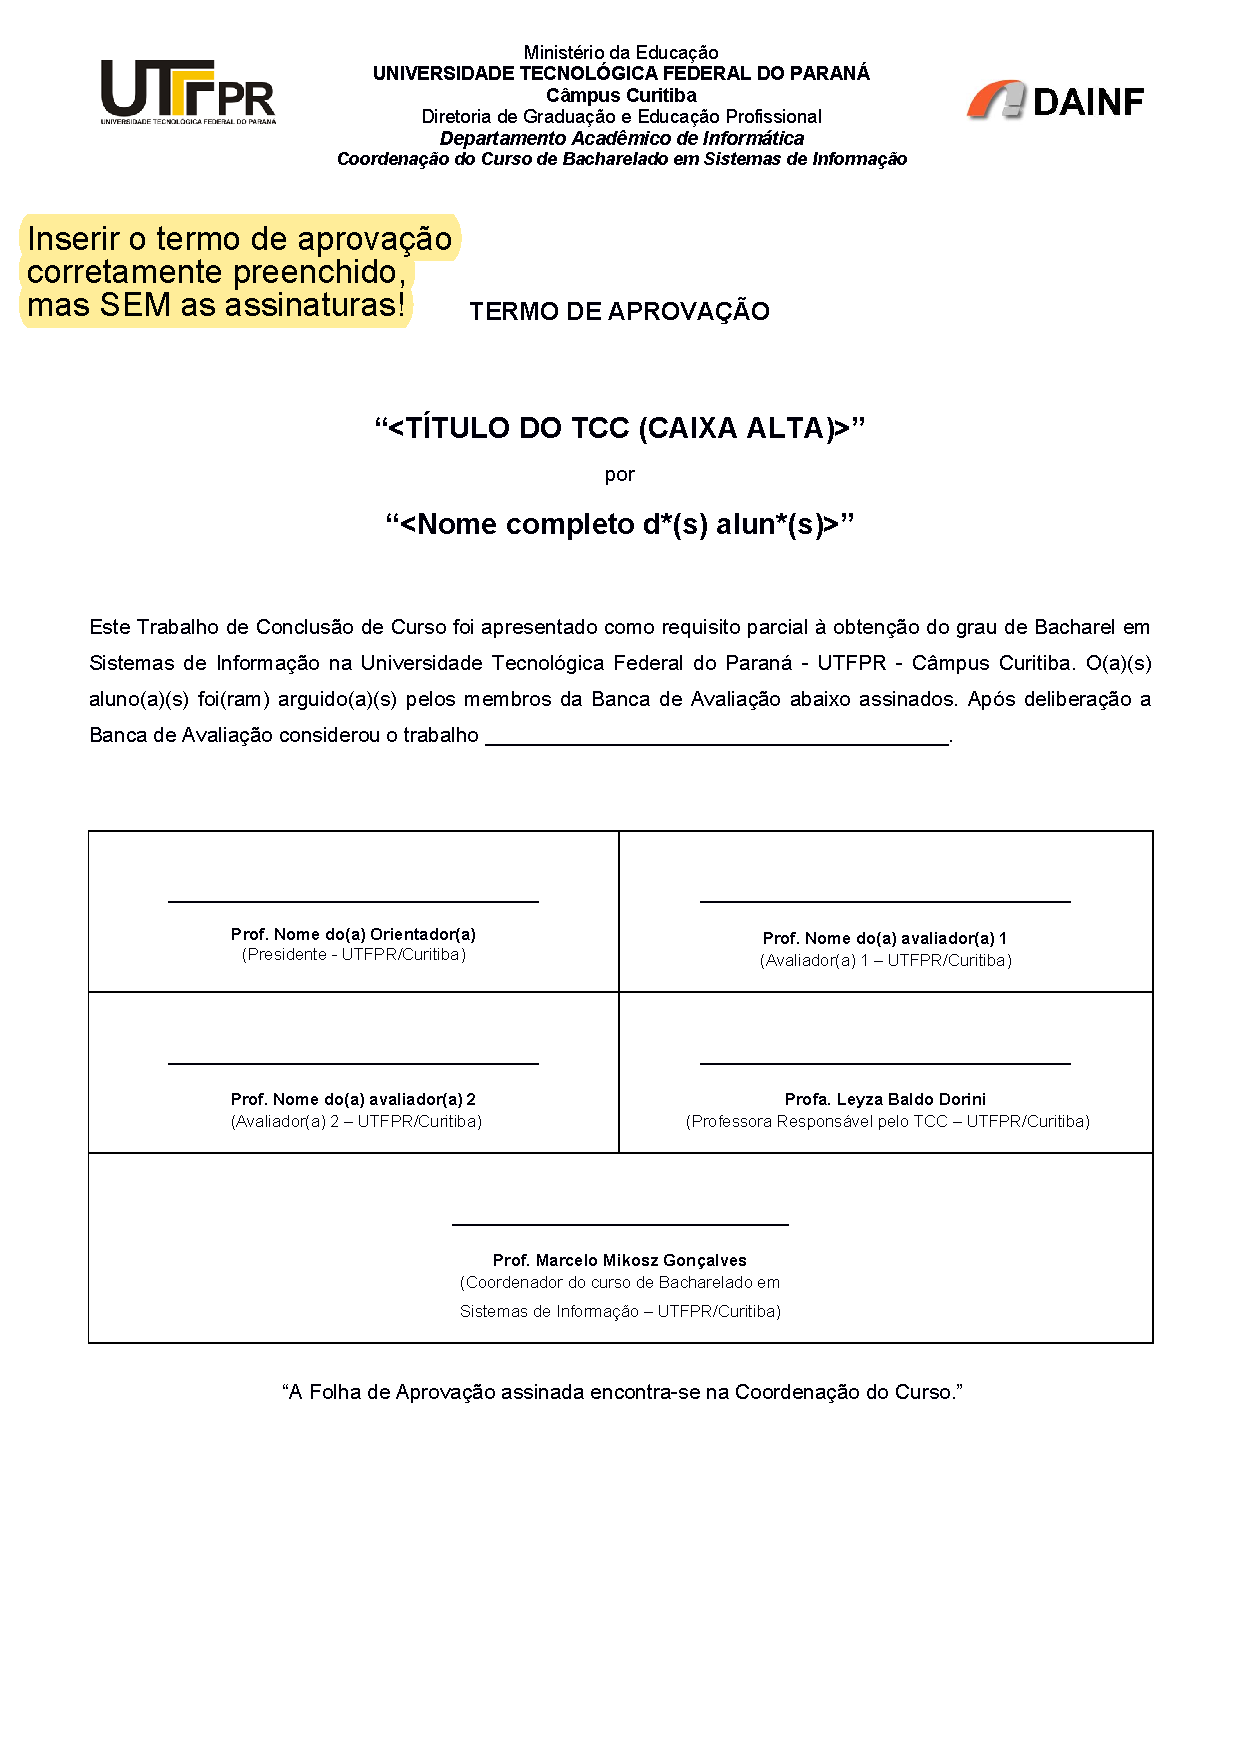
\includepdf[pages=-,pagecommand={},width=\textwidth]{dados/FOLHA_APROVACAO.pdf}

% RESUMO--------------------------------------------------------------------------------

\begin{resumo}[RESUMO]
\begin{SingleSpacing}

% Não altere esta seção do texto--------------------------------------------------------
\imprimirautorcitacao. \imprimirtitulo. \imprimirdata. \pageref {LastPage} f. \imprimirprojeto\ – \imprimirprograma, \imprimirinstituicao. \imprimirlocal, \imprimirdata.\\
%---------------------------------------------------------------------------------------

\lipsum[1] %trocar pelo resumo

\textbf{Palavras-chave}: Palavra1. Palavra2. Reconhecimento de padrões. 
% Escolha de 3 a 5 palavras ou termos que descrevam bem o seu trabalho 
\end{SingleSpacing}
\end{resumo}


             			   % Resumo em Português
%
% % ABSTRACT--------------------------------------------------------------------------------

\begin{resumo}[ABSTRACT]
\begin{SingleSpacing}

% Não altere esta seção do texto--------------------------------------------------------
\imprimirautorcitacao. \imprimirtitleabstract. \imprimirdata. \pageref {LastPage} f. \imprimirprojeto\ – \imprimirprograma, \imprimirinstituicao. \imprimirlocal, \imprimirdata.\\
%---------------------------------------------------------------------------------------

\lipsum[1] %trocar pelo abstract

\textbf{Keywords}: Word01. Word02. Pattern recognition. 
% Escolha de 3 a 5 palavras ou termos que descrevam bem o seu trabalho 

\end{SingleSpacing}
\end{resumo}


             		           % Resumo em Inglês
% % Lista de Figuras----------------------------------------------------------------

\pdfbookmark[0]{\listfigurename}{lof}
\listoffigures*
\cleardoublepage

% OBSERVAÇÕES---------------------------------------------------------------------
% Este arquivo não precisa de ser alterado, pois a lista é gerada automaticamente.
   % Lista de Figuras
%% LISTA DE QUADROS----------------------------------------------------------------

\renewcommand{\listofquadrosname}{LISTA DE QUADROS}

\pdfbookmark[0]{\listofquadrosname}{loq}
\listofquadros*
\cleardoublepage

% OBSERVAÇÕES---------------------------------------------------------------------
% Este arquivo não necessita de ser editado. A lista é gerada automaticamente.
   % Lista de Quadros
%% LISTA DE TABELAS-------------------------------------------------------------

\pdfbookmark[0]{\listtablename}{lot}
\listoftables*
\cleardoublepage

% OBSERVAÇÕES-------------------------------------------------------------------
% Este arquivo não precisa ser alterado, pois a lista é gerada automaticamente.
         		   % Lista de Tabelas
%$% LISTA DE ABREVIATURAS E SIGLAS----------------------------------------------------------

\begin{siglas}
  %  \item[PPGEB] Programa de Pós-Graduação em Engenharia Biomédica
    \item[GLCM] \textit{Gray-level Co-ocurrence Matrix}, do inglês matriz de coocorrência em escala de cinza
    \item[ROI] \textit{Region of Interest}, do inglês, região de interesse.
    \item[PROENG] Processamento e Análise de Imagens Aplicadas à Mastologia
    \item[UFF] Universidade Federal Fluminense
    \item[DMR] \textit{Database For Mastology Research}, do inglês, base de dados para pesquisa em mastologia
    \item[HPP] \textit{Horizontal Projection Profile}
    \item[SVM] \textit{Support Vector Machine}
 %   \item[SIBGRAPI] Conference on Graphics, Patterns and Images
\end{siglas}

% OBSERVAÇÕES-----------------------------------------------------------------------------
% Altere a lista acima para definir os acrônimos e siglas utilizados neste trabalho
          		   % Lista de Abreviaturas e Siglas
%% LISTA DE SÍMBOLOS------------------------------------------------------------

\begin{simbolos}
    \item[$ \Gamma $] Letra grega Gama
    \item[$ \lambda $] Comprimento de onda
    \item[$ \in $] Pertence
\end{simbolos}

% OBSERVAÇÕES-------------------------------------------------------------------
% Altere a lista acima para definir os símbolos utilizados no trabalho
        		   % Lista de Símbolos
%% LISTA DE ALGORITMOS----------------------------------------------------------

\newcommand{\algoritmoname}{Algoritmo}
\renewcommand{\listalgorithmcfname}{LISTA DE ALGORITMOS}

\floatname{algocf}{\algoritmoname}
\newlistof{listofalgoritmos}{loa}{\listalgoritmoname}
\newlistentry{algocf}{loa}{0}

\counterwithout{algocf}{chapter}
\renewcommand{\cftalgocfname}{\algoritmoname\space}
\renewcommand*{\cftalgocfaftersnum}{\hfill--\hfill}

\pdfbookmark[0]{\listalgorithmcfname}{loa}
\listofalgorithms
\cleardoublepage

% OBSERVAÇÕES------------------------------------------------------------------
% Este arquivo não precisa ser alterado, pois a lista é gerada automaticamente.
   % Lista de Algoritmos
% SUMÁRIO----------------------------------------------------------------------

\renewcommand{\contentsname}{SUMÁRIO}

\pdfbookmark[0]{\contentsname}{toc}
\tableofcontents*
\cleardoublepage

% OBSERVAÇÕES-------------------------------------------------------------------
% Este arquivo não precisa ser alterado, pois o sumário é gerado automaticamente.
               			   % Sumário

\textual
% INSERE ELEMENTOS TEXTUAIS




% INTRODUÇÃO-------------------------------------------------------------------

\chapter{INTRODUÇÃO}
\label{chap:introducao}

A popularização e o aperfeiçoamento das tecnologias digitais, juntamente com a disseminação da Internet, são frequentemente reconhecidos como elementos centrais para o progresso econômico, político e social do século XXI \cite{Silveira2021}. A interação contínua com dispositivos conectados tornou-se um aspecto essencial e recorrente na vida cotidiana das pessoas \cite{silveira-demcodigos}, e é nesse contexto que as plataformas digitais se consolidam como ambientes de intermediação, mediando cada vez mais aspectos da vida social e reconfigurando as atividades humanas, inserindo práticas cotidianas no contexto digital, um ecossistema profundamente conectado e orientado a dados. No entanto, esse processo não ocorre de forma neutra. 

As Tecnologias da Informação e Comunicação (TICs), ao serem apropriadas pela racionalidade neoliberal, tornam-se ferramentas que dominam a linguagem e moldam o ambiente digital de modo a favorecer interesses corporativos, transformando espaços diversos em organizações focadas no lucro, reproduzindo uma sociedade incivil, em que interesses privados se sobrepõem aos públicos, com tecnologias operadas por algoritmos que reduzem a diversidade das relações \cite{souza_sabbag_achilles_2024}. Por sua vez, esses algoritmos, essência constituinte das chamadas plataformas digitais, não têm intenção própria, isto é, eles operam por causas previamente explicitadas e não por fins conscientes. Mesmo que pareçam “inteligentes” ou “autônomos”, eles seguem regras e reações determinadas por sua programação inicial e infraestrutura física \cite{Faustino2023}. As plataformas digitais, como tecnologias, estão sujeitas a abarcarem propósitos para além de seu uso imediato \cite{Winner_2019}.

\sout{Este trabalho busca contribuir com o diálogo entre os saberes técnicos e humanísticos, uma vez que enxergo a lacuna existente hoje no que tange a ausência da dimensão humana na produção tecnológica, apontada por \citeonline{Faustino2023}.} [JUSTIFICATIVA]

\section{Pergunta de Pesquisa e Objetivos}
\label{sec:perg}
Analisar a atuação do Núcleo de Tecnologia do MTST como estratégia de soberania digital e resistência popular ao capitalismo de vigilância.

\subsection{Objetivos Específicos}
\label{subsec:objEs}

\section{Justificativa da Pesquisa}
\label{sec:just}

O projeto de pesquisa proposto se insere no cerne das disputas contemporâneas por soberanias digitais e busca compreender as formas de resistência e luta contra-hegemônica que emergem em um cenário de colonialismo digital e capitalismo de vigilância. Ao focar no Núcleo de Tecnologia do MTST (Movimento dos Trabalhadores Sem Teto), o estudo se dedica a analisar as dinâmicas digitais a partir de um saber localizado, como proposto por Donna Haraway e discutido por \citeonline{evangelista2017}.

\citeonline{evangelista2017} argumenta que os efeitos das tecnologias de vigilância e do Big Data não devem ser pensados como categorias universais, mas sim a partir das diferentes posições sociais. Ele fala como pesquisador de um país periférico ao sul do globo, preocupado com o destino de trabalhadoras e trabalhadores que vivem um cotidiano de crescente instabilidade econômica. Estudar o MTST permite analisar o capitalismo de vigilância e o colonialismo digital a partir da perspectiva e da experiência de um grupo socialmente vulnerável em um país periférico, o que, segundo o autor, nos obriga a pensar em especificidades e ênfases diferentes em relação à literatura vinda dos países centrais.

A importância do estudo também se fundamenta na crítica de \citeonline{Faustino2023} sobre o colonialismo digital, sendo o MTST um movimento social que já debate o tópico, buscando caminhos para a tecnopolítica e a descolonização da tecnologia. Além disso, o projeto aborda diretamente a problemática levantada pelos autores sobre o "abismo teórico que perpassa os dois polos" \cite[p.~30]{Faustino2023} entre a formação técnica e a humanística. Eles criticam a falta de compreensão da dimensão humana na produção tecnológica nos cursos técnicos e a superficialidade com que as ciências humanas tratam o funcionamento e atuação das tecnologias digitais. 

Estudar o Núcleo de Tecnologia do MTST oferece a oportunidade de compor essa interface de comunicação necessária ao analisar como um movimento social\footnote{Estou usando a denominação que eles empregam no site, mas trago o debate na próxima seção}, enraizado em lutas humanísticas e sociais, se apropria e se relaciona com as tecnologias digitais de forma crítica e estratégica. Isso permite ir além da mera denúncia do "fetiche da tecnologia" \footnote{Esses conceitos estão no livro de \cite{Faustino2023}, não sei se vou manter aqui na justificativa mesmo, se vou aprofundar eventualmente na revisão teórica} – a crença na neutralidade da técnica – e investigar as possibilidades de atuação política contra-hegemônicas, buscando "reintroduzir a política e a economia nesse debate sobre tecnologia" \footnote{Para retomar a discussão na revisão de literatura: \citeauthor{fisher_2020} levanta a questão de que  que nada é inerentemente politico. A politização requer um agente político que possa transformar o que é tido como garantido em algo a ser disputado. Essa questão é abordada no Cap. 2 do \cite{Silveira2021} também, checar fichamentos}.

\section{Organização do Trabalho}
\label{sec:org}
                		           % Introdução
% REVISÃO DE LITERATURA--------------------------------------------------------

\chapter{REVISÃO DE LITERATURA}
\label{chap:revisaodeliteratura}

\section{Do Colonialismo Histórico ao Capitalismo de Vigilância}
\label{sec:colDigital}

Para abordar o tema do colonialismo digital e compreender suas características e formas de atuação na contemporaneidade, é fundamental, antes de qualquer coisa, realizar um resgate histórico do conceito de colonialismo em si. Essa contextualização inicial me parece indispensável para que possamos estabelecer as conexões necessárias entre os mecanismos de dominação do passado e suas ressignificações nas estruturas digitais atuais.

Segundo \citeonline{quijano2005}, o conceito tradicional de colonialismo, entendido como dominação política direta de um território por uma potência externa, é insuficiente para capturar a complexidade e a durabilidade dos padrões de poder estabelecidos a partir da conquista da América. A  colonização das Américas dá origem à ideia de raça como conhecemos hoje; as relações sociais que se fundamentam nessa base produzem na América novas identidades, bem como redefinem identidades já existentes. É nesse contexto que nascem o índio, o negro e o mestiço — e que renascem o  português, o espanhol e o europeu. 

Para além da procedência geográfica, esses termos agora adquirem uma conotação racial e são associados a identidades hierarquizadas dentro de um contexto de dominação, identidades essas que passam a ser associadas à natureza dos papéis na estrutura global de controle do trabalho. Dessa forma, é imposta uma sistemática divisão racial do trabalho: formas de trabalho forçado e não remunerado foram adscritas aos não-brancos nas colônias, enquanto o trabalho livre assalariado ficou limitado à raça colonizadora, brancos europeus \cite{quijano2005}. 

Ainda segundo o autor, todas as formas de controle do trabalho na América foram deliberadamente estabelecidas e organizadas em torno e em função do capital e é essa realidade que fornece a base material para a acumulação primitiva europeia através do saque nas colônias, o que constitui então o capitalismo mundial e a Europa no centro desse novo sistema. Este processo estabelece um controle eurocêntrico dos mercados mundiais, fazendo da exploração colonial uma condição de existência do capitalismo \cite{quijano2005}.

Esta perspectiva nos ajuda a consolidar um entendimento sobre a continuidade dos padrões de dominação na era pós-colonial, pois, enquanto o colonialismo político tem duração limitada no tempo e termina com a independência formal, a colonialidade perdura após a independência política, reproduzindo-se estruturalmente nas sociedades contemporâneas. É neste padrão de poder mundial que a hegemonia de instituições específicas molda diversos âmbitos da existência social: a empresa capitalista controla o trabalho, a família burguesa articula as relações de sexo/gênero, o Estado-nação define a autoridade e, por fim, o eurocentrismo influencia a intersubjetividade
\cite{quijano2005}.

A colonialidade do poder é, portanto, fundamental para explicar a elaboração e hegemonia dessa perspectiva eurocêntrica sobre a subjetividade do colonizado\footnote{
Duas das características do colonialismo digital remontam mais diretamente ao colonialismo histórico, por se tratar de um controle material sobre recursos/territórios colonizados (controle da infraestrutura, controle da extração de minérios), mas, quando falo de colonialismo de dados e, mesmo, de capitalismo de vigilância, acho que é importante fundamentar a perspectiva de controle de subjetividades pelo eurocentrismo, por isso o conceito de colonialidade do poder casa bem aqui. Acho que vou retomar essa discussão ainda.
}, uma vez que se apresenta como a imposição de modelos de pensamento, de agenciamentos, de comportamentos que negam ou desvalorizam diferentes saberes, modos de aprender e conhecer das comunidades e das sociedades não ricas \cite{Silveira2021}.

Além da colonização das Américas, o colonialismo apresenta outras duas fases distintas: a colonização da Ásia e da África, cujas lutas por libertação se intensificaram após a Segunda Guerra Mundial, impulsionadas pelo enfraquecimento das potências europeias. \cite{beuron2024}. E, também, uma terceira forma de colonialismo que emerge a partir do fim da Guerra Fria, com a consolidação do ordenamento neoliberal, que amplia e aprofunda a colonialidade, e o avanço das tecnologias informacionais: o colonialismo de dados \cite{beuron2024, Silveira2021}.

\subsection{Colonialismo Digital}
\label{subsec:colDigital}

O colonialismo de dados surge como um dos elementos que constituem, juntamente com a nova repartição do mundo em espaços de exploração econômica, o que \citeonline{Faustino2023} definem como colonialismo digital, uma nova dinâmica do capitalismo tardio que engloba diversas dimensões da dominação e exploração contemporânea mediada pela tecnologia. Para os autores, não se trata de uma fase pós-capitalista ou um novo modo de produção, mas sim uma rearticulação de velhas formas de exploração sob o contexto de uma sociedade em que a alta tecnologia convive com as mais baixas condições de vida.

A nova repartição territorial do globo terrestre em espaços de exploração econômica, como um dos dois elementos intercambiáveis constituintes do colonialismo digital, atualiza o imperialismo, subimperialismo e neocolonialismo tardio, reduzindo o chamado Sul Global a um "mero território de mineração extrativista de dados informacionais". Isso envolve a concentração de capital, recursos intelectuais e infraestrutura material (como cabos, servidores e data centers) em poucos países. Também inclui a extração de matérias-primas (ouro, lítio, coltan) necessárias para o hardware \cite{Faustino2023}.

A rede de cabos submarinos, por exemplo, é parte da infraestrutura material essencial para a expansão e manutenção da rede digital. Junto com data centers e torres de transmissão, ela distribui o fluxo de dados globalmente \cite{Figueiredo2023}, parte do que \apudonline{Couldry2019}{Figueiredo2023} chamam de "Império da Nuvem". 

% Este "império" é impulsionado por corporações, notadamente ocidentais, mas também chinesas, e faz das seguintes forças: 
% \begin{enumerate}
%     \item \textbf{Infraestrutura de extração de dados:} Base tecnológica em constante expansão, voltada à coleta massiva de informações.
%     \item \textbf{Ordem social emergente:} Conecta os seres humanos a essas infraestruturas, moldando novas formas de interação e controle.
%     \item \textbf{Modelo de governança social:} Atua para integrar ainda mais os indivíduos a esse sistema, explorando suas conexões com a infraestrutura e a nova ordem social.
%     \item \textbf{Racionalidade prática:} Confere sentido e legitimidade a esses processos, orientando ações e decisões dentro dessa lógica.
%     \item \textbf{Modelo de conhecimento:} Redefine o mundo partindo da premissa de que os dados seriam capazes de explicar tudo o que existe e de dar conta de todo o conhecimento possível.
% \end{enumerate}

Ao lado dessa reconfiguração dos espaços de exploração econômica promovida pelas grandes corporações tecnológicas, se configura, por fim, o colonialismo de dados, segundo elemento constitutivo do colonialismo digital.

\subsection{Colonialismo de Dados}
\label{subsec:colDados}

Para \citeonline{couldry2018} e \citeonline{Silva2023}, assim como o colonialismo histórico se apropriou de território, recursos naturais e corpos, o colonialismo de dados se apropria da vida em geral e a anexa ao capital, combinando as práticas extrativas predatórias do colonialismo tradicional com os métodos abstratos de quantificação da computação, transformando a experiência cotidiana em insumo para a geração de valor econômico. Para isso, as mesmas racionalidades extrativistas precisam ser naturalizadas ou normalizadas e, assim, o  colonialismo de dados constrói os dados\footnote{
Por dados, entende-se as medições ou observações que são coletadas como uma fonte de informação. A natureza dos dados pode variar amplamente, existindo diferentes tipos e formas de representação \cite{data_2025}.
} como "matéria-prima natural", apagando os processos de apropriação subjacentes.

Segundo os autores, esse é um processo que vai além da simples ideia de que "dados são o novo petróleo"\footnote{
A expressão "dados são o novo petróleo" foi cunhada por Clive Humby, em 2006, sugerindo que os dados possuem um valor econômico significativo. Humby, um matemático britânico, obteve sucesso financeiro através do gerenciamento de "big data". \cite{arthur_2013}.
}, pois, ao contrário do petróleo, os dados não são encontrados na natureza, mas precisam ser apropriados. Ele se manifesta através de "relações de dados", novos tipos de relações humanas que permitem a extração de dados para a \textit{commoditização}. Essencialmente, trata-se da transformação da vida cotidiana em um fluxo contínuo de dados que estarão sempre à mercê do capital. As plataformas digitais\footnote{\label{nota:plataformasDigitais}
Referência às grandes corporações tecnológicas que operam como intermediárias centrais da vida social online, capturando dados e moldando interações com fins econômicos. Entre essas corporações destacam-se as reunidas no acrônimo GAFAM — Google, Apple, Facebook (hoje Meta), Amazon e Microsoft —, que dominam o ecossistema digital ocidental \cite{couldry2018, Silveira2021, Reis2024, röhe_2024}. Há também gigantes do setor na China, como Baidu, Alibaba e Tencent \cite{couldry2018}, mas no contexto brasileiro, as plataformas de origem norte-americana exercem impacto mais significativo sobre a dinâmica social, econômica e informacional.
}, por sua vez, são o meio tecnológico que produzem esse novo "social" em uma forma que pode ser rastreada, capturada, classificada e contada como dado. 

Se, com o advento do capitalismo industrial, o trabalho é transformado em uma forma social abstrata e adquire uma dimensão mensurável que vai permitir sua troca no mercado, no contexto do colonialismo digital, a interação social comum passa a ser um fator de produção cujo dado pode ser apropriado e abstraído, transformando a vida humana em geral em uma nova forma social abstrata pronta para ser mercantilizada. Desta forma, muitos outros aspectos da vida além do trabalho passam a ser considerados relações econômicas \cite{couldry2018}.

O colonialismo de dados envolve ao menos dois polos de poder: os Estados Unidos e a China \cite{couldry2018}, que, apesar de ter sido historicamente vítima do colonialismo europeu, hoje assume um papel de protagonismo econômico global \cite{Silveira2021}.  Para a China, os dados são considerados um fator de produção chave e estratégico que impulsiona o crescimento econômico e tem um impacto significativo na alocação de recursos sociais e na lógica das operações econômicas e sociais \cite{feifei2024}.


Colonialismo de dados é, portanto, uma estrutura real que recria relações desiguais entre países ricos (Norte Global) e pobres (Sul Global), em que os fluxos de dados, vistos como insumo e capital, são extraídos predominantemente das periferias em direção às corporações tecnológicas concentradas no Norte. Esses dados são, então, usados para gerar riqueza, mas essa riqueza vai para as corporações e países que os coletam, e não para o país de origem dos dados \cite{Silveira2021}.

Neste cenário, a partir de 2019 e durante o governo de Donald Trump nos EUA, o Brasil adotou uma política externa marcada por subserviência deliberada aos interesses norte-americanos e passou a seguir de forma quase automática as posições de Washington, mesmo com os produtores de tecnologia\footref{nota:plataformasDigitais} demonstrando pouco interesse real nas necessidades e condições dos consumidores periféricos, exceto quando isso serve para aprimorar seus próprios produtos com base em feedback ou explorar nichos de mercado que ofereçam lucro \cite{Silveira2021}.

Esse alinhamento automático às diretrizes dos centros tecnológicos globais evidencia não apenas uma dependência política, mas também uma inserção subordinada na lógica do capitalismo de dados, o que permite compreender como se articulam, nesse contexto, o colonialismo de dados e sua face operacional mais visível: o capitalismo de vigilância.

\subsection{Capitalismo De Vigilância}
\label{subsec:capVigilancia}

\citeonline{Zuboff2019} define o Capitalismo de Vigilância como um modelo de negócios em que a experiência humana é traduzida em dados comportamentais para prever e direcionar ações futuras, e o direito à privacidade é usurpado por reivindicações unilaterais do mercado. As plataformas digitais se apropriam da experiência do usuário como matéria-prima gratuita, extraindo dados de suas interações, preferências e comportamentos. Neste modelo, o comportamento humano é arrebanhado em busca de resultados lucrativos e os meios de produção são subordinados aos "meios de modificação comportamental"; os clientes deixam de ser os seres humanos, que viram objetos de extração de matéria-prima, e se tornam as próprias empresas.

Vale ressaltar que o emprego do termo não é consenso entre todos os autores que discorrem sobre o tema, \citeonline{Faustino2023}, por exemplo, ressaltam que analisar esses processos sob a ótica do surgimento de uma nova lógica de acumulação sem precedentes pode ignorar ou secundarizar alguns conceitos que auxiliariam na análise histórica do problema, o que fragiliza o debate e a percepção do que permanece do período anterior, embora agora intensificado ou reconfigurado com as novas possibilidades tecnológicas. \citeonline{Zuboff2019}, por sua vez, argumenta que o Capitalismo de Vigilância escapa das lentes analíticas tradicionais — como monopólio, privacidade ou mesmo vigilância estatal — tornando-se difícil de ser plenamente compreendido e enfrentado. Por ser sem precedentes, tende a ser interpretado como uma extensão de fenômenos conhecidos, o que obscureceria seu caráter original e radical.

Há, ainda, uma tendência, inclusive estimulada pelos próprios atores do setor, de confundir o Capitalismo de Vigilância com as tecnologias que o viabilizam (como algoritmos, plataformas ou inteligência artificial). No entanto, a autora enfatiza que o Capitalismo de Vigilância é uma lógica de mercado que utiliza essas tecnologias, mas não se reduz a elas. Essa confusão serve para naturalizar e legitimar práticas de extração de dados como se fossem inevitáveis, quando, na verdade, são escolhas políticas e econômicas\citeonline{Zuboff2019}.

A ideologia\footnote{
A ideologia pode ser entendida como um tecido de ideias e conceitos, um sistema de ideias ou uma visão filosófica que serve a propósitos sociais e políticos específicos,  está intrinsecamente ligada aos interesses de classe e de nação \cite{vieirapinto1963}.
} exerce papel central no funcionamento e na legitimação do Capitalismo de Vigilância e do Colonialismo de Dados. O sucesso e a expansão dessas formas de dominação digital dependem de um conjunto de crenças, narrativas e justificativas que naturalizam práticas de extração e controle de dados, tornando-as não apenas aceitáveis, mas desejáveis ou inevitáveis para a sociedade \cite{Zuboff2019}. Esse processo é amplificado por uma lógica tecnossolucionista, que promove a ideia de que problemas sociais complexos podem ser resolvidos por meio da implementação de soluções tecnológicas, promovendo a ilusão de neutralidade tecnológica e mascarando interesses econômicos e políticos por trás das inovações digitais, o que reforça a dependência de países periféricos em relação às soluções produzidas pelo Norte Global, além de perpetuar desigualdades e opressões históricas \cite{Faustino2023}.

Essa lógica se fundamenta no que \citeonline{barbrook1995} definiram como Ideologia Californiana, que surge no Vale do Silício e é impulsionada por uma profunda fé no potencial emancipador das novas tecnologias da informação. Acreditava-se que as novas tecnologias de informação emancipariam o ser humano, ampliando a liberdade individual e reduzindo o poder do "Estado burocrático".

Ademais, a ideologia neoliberal também é fundamental para criar o ambiente no qual o colonialismo de dados prospera. Ela promove valores como a desregulamentação, a centralidade do mercado e a responsabilização individual, enfraquecendo mecanismos coletivos de resistência e regulação. Assim, a ideologia atua tanto para mascarar as relações de dominação quanto para justificar a ausência de alternativas, reforçando a sensação de inevitabilidade tecnológica e de dependência em relação às grandes plataformas globais \cite{Faustino2023}.
% Capitalismo de Plataformas\footnotemark[\value{footnote}] é definido como um capitalismo de dados tratados por algoritmos. 

% Com a redução dos custos de computação e armazenamento de dados, aliada à consolidação da comunicação digital, Srnicek aponta a abertura de um novo potencial para o desenvolvimento de produtos e serviços orientados à extração de informações. Esses dados passaram a ser utilizados em processos produtivos, na identificação das preferências dos consumidores e no controle tanto dos trabalhadores quanto das cadeias logísticas \cite{silveira-demcodigos}. 

% O armazenamento massivo de dados permite que desenvolvedores de algoritmos infiram categorias identitárias a partir dos hábitos de navegação dos usuários na internet, especialmente quando essas informações são cruzadas com outras bases de dados \cite{silveira-demcodigos}\footnote{Isso é na verdade uma paráfrase da frase original, que está na página 25: 
% "O armazenamento de grande quantidade de dados oferece aos desenvolvedores de algoritmos a condição de inferir categorias identitárias baseadas nos hábitos de navegação na internet e no cruzamento com outras informações.". Achei interessante colocar aqui, mas não sei ainda se vou usar. Na minha visão, não são exatamente os desenvolvedores que inferem categorias identitárias — são os algoritmos, programados por eles, que realizam inferências com base nos dados. Embora os algoritmos sejam programados por desenvolvedores, esses profissionais não possuem acesso direto aos dados utilizados nem controle sobre os processos de inferência automatizada. Assim, a extração de perfis identitários é realizada por sistemas opacos cuja lógica de funcionamento escapa, em muitos casos, até mesmo àqueles que os constroem. Nesse mesmo livro o autor discute a questão da opacidade algorítmica: no primeiro capítulo, ao mencionar Lucas Introna e a ideia de que, mesmo com acesso ao código-fonte, é impossível compreender plenamente o funcionamento dos algoritmos. Posteriormente, no Cap. 4, aborda como as Big Techs intensificam essa opacidade ao manterem seus códigos proprietários fechados, dificultando ainda mais a transparência e a auditoria pública.}.


Por fim, destacam-se algumas características intrínsecas do Colonialismo Digital: 

\begin{enumerate}
    \item \textbf{Oligopólios das Big Techs:} Grandes corporações, predominantemente do Vale do Silício, controlam setores estratégicos da indústria da informação, como aplicativos e serviços em nuvem, acumulando trilhões em receitas e monopolizando o acesso a dados \cite{Faustino2023, Silva2023, furtado2024, couldry2018, Zuboff2019}.
    \item \textbf{Mineração de Dados no Sul Global:} Países do Sul Global se tornam "territórios de mineração extrativista de dados", servindo como fonte de matéria-prima digital e consumidores de "manufaturados pós-modernos" \cite{Faustino2023, furtado2024, Silveira2021, Silva2023}.
    \item \textbf{Subsunção da Vida Humana:} Exploração do ócio, da a criatividade e da cognição, transformando a experiência humana em "matéria-prima" para a acumulação de capital. A vida é cada vez mais convertida em uma "coleção de mercadorias"\cite{Faustino2023, couldry2018, Silveira2021, Zuboff2019}..
    \item \textbf{Infraestrutura Material e Extrativismo Tradicional:} A existência do mundo digital depende de uma vasta infraestrutura física, como cabos de fibra óptica e datacenters. Isso impulsiona a extração violenta de minérios essenciais (lítio, coltan) de regiões como a África e a América Latina, replicando o extrativismo colonial \cite{Faustino2023, Figueiredo2023}.
    \item \textbf{Racialização Digital:} O racismo é reproduzido e ampliado por algoritmos e sistemas de inteligência artificial, que incorporam vieses discriminatórios e reforçam a seletividade racial no acesso e uso da tecnologia. Isso cria novas hierarquias "bioeconomicorraciais" \cite{Faustino2023}.
    \item \textbf{Privatização da Soberania:} Há uma crescente privatização do poder, com as Big Techs exercendo influência política e econômica sobre os Estados-nação, inclusive em eleições \cite{Faustino2023}.
\end{enumerate}

Diante deste cenário, a resistência é um tema central e multifacetado, envolvendo tanto dimensões técnicas quanto políticas, sociais e epistêmicas.

\section{Resistência}
\label{sec:resitencie}

Para os autores \citeonline{Silveira2021} a resistência é compreendida como um movimento que precisa ir além das respostas jurídicas ou regulatórias tradicionais. Eles enfatizam a necessidade de ações coletivas, de alternativas tecnológicas baseadas em princípios de soberania digital, transparência, controle social e desenvolvimento de infraestruturas próprias, especialmente nos países do Sul Global. A obra apresenta exemplos concretos, como o desenvolvimento da criptomoeda indígena Oyxabaten, criada por comunidades de Rondônia e Mato Grosso do Sul, como uma experiência de apropriação tecnológica local que visa à subsistência econômica e à autonomia diante do abandono estatal durante a pandemia de Covid-19. Os autores defendem que resistir ao colonialismo de dados exige pensar alternativas que partam das realidades e necessidades locais, rompendo com o universalismo tecnocientífico imposto pelas Big Techs e pelo Norte Global.

\citeonline{Faustino2023} abordam a resistência inspirando-se nas lutas anticoloniais de Frantz Fanon. Para eles, a resistência ao colonialismo digital e de dados implica desvelar e enfrentar as ideologias que sustentam a dominação tecnológica, como o fetichismo da técnica\footnote{O fetichismo da tecnologia (ou fetichismo da técnica) é um conceito que se relaciona diretamente com o fetichismo da mercadoria de Karl Marx. Assim como no fetichismo da mercadoria, em que objetos inanimados parecem ter vida própria, o fetichismo da tecnologia ocorre quando a tecnologia parece ter ânima, vida ou consciência. Esse fenômeno acaba escondendo o trabalho humano contido nessas tecnologias \cite{Faustino2023}}, a ilusão da neutralidade tecnológica e o tecnossolucionismo. Os autores sugerem que a resistência pode se dar por meio da reapropriação, recusa ou reinvenção das tecnologias, bem como pelo fortalecimento de laboratórios de periferia, clubes hacker, cooperativismo de plataforma, letramento crítico e pedagogias alternativas.

\citeonline{couldry2018}, por sua vez, sugerem que a resistência a essa nova forma de colonialismo deve se basear no pensamento decolonial, inspirado em sociólogos como Aníbal Quijano. A essência da resistência, segundo os autores, é atacar o núcleo da racionalidade subjacente que permite que a apropriação contínua de dados pareça natural, necessária e até mesmo benéfica para o desenvolvimento humano, em vez de uma violência. A resistência deve também rejeitar a ideia de que os resultados do processamento de dados são uma forma de conhecimento social que ocorre naturalmente, reconhecendo-os como uma forma de extração motivada comercialmente que avança interesses econômicos e/ou de governança específicos. Um primeiro passo útil seria nomear a prática contemporânea de apropriação de dados como o processo colonial que ela é.

\citeonline{Souza2024} propõem o "comum" como forma de resistência à ordem neoliberal e ao controle das Big Techs. Os autores questionam a previsibilidade total e o domínio das redes, que redefinem o espaço vital em esfera virtual e desconstroem mediações sociais tradicionais. Sugerem, então, repensar o espaço político do comum, entendendo a comunicação como partilha simbólica que possibilita o "ser-em-comum".

A soberania digital, como um conceito também multifacetado, configura-se como um eixo central de resistência ao colonialismo de dados e à dependência tecnológica imposta pelas grandes corporações.

\subsection{Soberania Digital}
\label{subsec:soberania}
O conceito de soberania possui várias interpretações, mas pode ser compreendido, em linhas gerais, como um processo de legitimação jurídica do poder — a conversão da força bruta em autoridade reconhecida \cite{lemos2024}. Em episódio de seu podcast \citeonline{tecnopolitica2023}, Sérgio Amadeu contextualiza o termo historicamente, destacando que sua formulação original remonta a Jean Bodin, que definia soberania como a capacidade dos governos exercerem sua autoridade de forma autônoma dentro de seu território, uma concepção alinhada ao contexto absolutista de sua época.

Com o avanço das ideias liberais e iluministas, o conceito de soberania passou por transformações significativas. Jean-Jacques Rousseau desenvolveu a noção de soberania popular, segundo a qual o poder exercido pelo governo deve, necessariamente, emanar do povo.Em contraposição, Carl Schmitt formulou a ideia de que soberano é aquele que detém o poder de declarar o estado de exceção. Essa concepção, frequentemente associada a regimes autoritários, é utilizada para sustentar teorias políticas não democráticas e totalitárias \cite{tecnopolitica2023}.


O território como espaço físico, onde se aplicam as leis e o poder soberano de cada Estado, está, portanto, associado ao exercício da soberania estatal. A internet, por sua vez, apesar de representar um espaço virtual,  depende intrinsecamente de cabos de fibra óptica, servidores, data centers e outros equipamentos que estão localizados nesses territórios físicos; desta forma, as atividades online, as empresas que operam na internet e os dados em circulação estão ancorados em uma infraestrutura material, o que nos faz descartar a ideia de que a internet estaria livre da soberania dos países, uma vez que esta não se sustenta empiricamente  \cite{tecnopolitica2023}.

Com o surgimento de novas formas de poder e a atuação de diferentes agentes de influência ao longo da história, dentre eles as chamadas Big Techs, os campos político e jurídico foram desafiados a reavaliar o conceito tradicional de soberania \cite{lemos2024}. Nesse novo cenário, o termo passa a assumir diferentes interpretações, dando origem a noções como soberania digital e soberania de dados \cite{tecnopolitica2023}, que refletem os embates contemporâneos em torno do controle sobre as infraestruturas tecnológicas e informacionais.

Talvez devido ao seu recém-surgimento, não há consenso sobre a definição objetiva dos conceitos ligados à soberania no contexto das redes. De acordo com a revisão sistemática de literatura realizada por \citeonline{lemos2024}, os termos “soberania digital”, “soberania dos dados” e “soberania de dados” passaram a circular com maior frequência na produção acadêmica brasileira a partir de 2022, mas não de maneira muito expressiva, embora os autores não descartem a possibilidade de conceitos análogos estarem sendo aplicados. Assim, o número reduzido de publicações com o uso direto do termo "soberania digital" poderia indicar a necessidade de um alicerçamento conceitual mais sólido nessa área \cite{lemos2024}.

A análise dos artigos revisados por \citeonline{lemos2024} revela que, embora não haja uma definição única de soberania digital, o conceito é mobilizado com sentidos convergentes, relacionados à autonomia, controle e regulação sobre infraestruturas, tecnologias e dados no ambiente digital. Enquanto no contexto da União Europeia o foco recai sobre a proteção de dados, a segurança cibernética e a construção de uma indústria tecnológica autônoma frente à hegemonia de empresas estrangeiras, na América Latina — especialmente em iniciativas brasileiras, argentinas e mexicanas — a soberania digital é associada à resistência ao domínio corporativo, à defesa da privacidade e ao desenvolvimento de tecnologias comunitárias e contra-hegemônicas. 

Em ambos os contextos, a soberania digital aparece como resposta à centralização de poder nas grandes corporações tecnológicas, mas difere quanto aos sujeitos políticos a que se refere: no norte global, Estados e blocos econômicos; no sul global, coletivos, comunidades e movimentos sociais. Assim, como resultado desta análise, os autores propõem uma definição do conceito de soberania digital:

\begin{quote}
Soberania digital é a capacidade de Estados e comunidades de exercer controle autônomo sobre tecnologias, infraestruturas digitais e dados, garantindo a proteção da privacidade, a segurança das informações e a governança independente, resistindo à dominação de grandes corporações e potências estrangeiras, e promovendo a autodeterminação no espaço digital. \cite{lemos2024}
\end{quote}

Portanto, sob a perspectiva do Sul Global, a soberania digital como um projeto político envolveria romper com acordos que priorizam Big Techs em detrimento de sistemas públicos \cite{Souza2024}, isto é, a priorização de contratos com empresas locais, bem como a criação de redes comunitárias de internet e a regulação de plataformas globais (como proposto no Marco Civil da Internet) \cite{silveira-demcodigos}. Neste sentido, o MTST e seu Núcleo de Tecnologia se mostram como agentes de resistência multifacetada frente ao avanço do colonialismo de dados, da plataformização do trabalho e das desigualdades digitais.

\subsection{O Movimento dos Trabalhadores Sem Teto }
\label{subsec:mtst}

Segundo informações disponíveis no próprio site da instituição, o Movimento dos Trabalhadores Sem Teto (MTST) é um movimento social urbano fundado em 1997 com o objetivo inicial de garantir o direito constitucional à moradia digna para todas as pessoas, estando presente em 14 estados brasileiros \cite{mtst_2024}. Sua principal forma de luta são as ocupações de terras que não cumprem função social nas periferias dos grandes centros urbanos \cite{mtst2023cartilha}.

De acordo com cartilha publicada no site do Núcleo de Tecnologia do MTST, o movimento teve origem a partir das experiências do Movimento dos Trabalhadores Rurais Sem Terra (MST), adaptando sua atuação às demandas do contexto urbano. No entanto, essa referência às origens não é mencionada no site oficial do MTST. Conforme a tese de doutorado da pesquisadora Débora Goulart, esse vínculo histórico também estava presente em uma outra cartilha, intitulada Cartilha do Militante, publicada em 2005 e atualmente indisponível online. Nessa publicação, o MTST reconhecia o MST como coautor de sua formação \cite{goulart2011anticapitalismo}. Apesar das diferentes interpretações sobre a origem do movimento, militantes do MTST confirmam o vínculo com o MST na sua criação, e é a partir de 2003 que o MTST se forma como um movimento autônomo em relação ao MST, com instâncias próprias  \cite{goulart2011anticapitalismo}.

Em sua tese, \citeauthor{goulart2011anticapitalismo} ressalta que o MTST se autorrefere como um movimento popular cujo elemento central é a classe, sendo uma organização dos trabalhadores. Em 2009, ele negava a alcunha de "movimento social" no sentido dado pela sociologia que, segundo eles, abarca praticamente qualquer tipo de mobilização, o que poderia esvaziar o caráter político e estruturante das lutas populares organizadas por trabalhadores. No entanto, em 2025, observa-se uma mudança de posicionamento: o próprio site do MTST refere-se ao grupo como um "movimento social" \cite{mtst_2024}. 

O movimento se considera legalista \cite{mtst2023cartilha}, ao fundamentar sua atuação na exigência de que os imóveis cumpram a função social prevista na Constituição Federal. Nos termos dos artigos 6º e 23, a moradia é reconhecida como um direito social e uma obrigação do Estado \cite{constituicao1988}. O projeto político do MTST é anticapitalista e antineoliberal. Ele busca a contestação do capitalismo por meio de lutas de ação direta, e entende a sociedade brasileira como capitalista onde opera a luta de classes. O movimento posiciona-se em oposição à exploração e dominação capitalista \cite{goulart2011anticapitalismo}.

Entre seus objetivos e atuações, além da moradia, destacam-se o combate à fome através do projeto Cozinhas Solidárias, que oferece alimentação diária e gratuita, utilizando recursos de hortas urbanas e doações. Eles oferecem diversas iniciativas de capacitação e assistência, como oficinas de construção de cisternas, cursos comunitários, oficinas de foto e vídeo, saraus e mutirões de assistência médica e jurídica \cite{mtst2023cartilha}.

A estrutura organizacional do MTST é composta por coletivos políticos e coletivos setoriais. As decisões estratégicas são formuladas nos coletivos políticos, enquanto os setoriais são responsáveis por implementá-las em suas respectivas áreas temáticas. Atualmente, o movimento conta com 13 setores, entre eles: Arquitetura, Arte e Cultura, Comunicação, Educação, Horta e Segurança Alimentar, Jurídico, Finanças e Captação de Recursos, Formação Política, Autodefesa, Organização, Negociação, Saúde e Assistência Social, além do Núcleo de Tecnologia, foco deste estudo \cite{mtst2023cartilha}.


\subsection{O Núcleo de Tecnologia}
\label{subsec:nucleotec}

A origem do núcleo se deu durante o momento de fortes tensões políticas marcadas pelas eleições presidenciais de 2018 e esteve ligada à percepção, por parte de profissionais de tecnologia na base do movimento, de que o bolsonarismo tinha um enraizamento social real, e não se resumia apenas à presença de robôs nas redes sociais \footnote{Contextualizar o momento histórico aqui, com a onda "robôs" do Bolsonaro. A cartilha dá a entender que nem todos enxergavam a atuação dos bolsonaristas nas redes como um movimento organizado, subestimavam a ameaça direta à democracia. }. Essa percepção catalisou debates internos sobre o papel estratégico da tecnologia na organização política, culminando na formalização do núcleo como um coletivo setorial dedicado a iniciativas tecnológicas \cite{mtst2023cartilha}.

Um primeiro passo foi a criação de um curso para desenvolvedores. Somado a isso, surgiram solicitações internas para a automação de tarefas cotidianas, como a conexão entre simpatizantes do movimento e trabalhadores da base que oferecem serviços sob demanda. Isso levou à criação do Contrate Quem Luta (CQL), um chatbot de WhatsApp que automatiza essa conexão. A escolha do WhatsApp como plataforma visou superar obstáculos enfrentados pelos trabalhadores da base, como smartphones com pouco espaço de armazenamento e acesso limitado à internet, aproveitando a gratuidade de tráfego de dados (zero rating) oferecida pelas empresas de telefonia \footnote{A justificativa é super valida, mas linkar aqui talvez com as problemáticas levantadas em \cite{Silveira2021} e \cite{Faustino2023}, WhatsApp é da Meta que tem a iniciativa Internet.org, que é basicamente uma estratégia de expansão do colonialismo digital, para colonizar a infraestrutura e o acesso digital, capturar dados >massivamente< e transformar a vida humana em ativos comercializáveis (mineração de dados, criação de perfis, etc.) e, assim, gerar lucro e exercer controle, tudo sob o pretexto de oferecer conectividade e conveniência (tem algo que é meio que institucionalizado, "plano de governo" mesmo, em cartilha formalizada pelo MIT(?) e seguida por governos mundo a fora, no sentido de transformação digital, checar nos fichamentos.}.

O Núcleo também atua no combate à desinformação no ambiente digital e contribuiu para a elaboração de documentos importantes como o Plano de Ação para o Cooperativismo de Plataformas no Brasil e o Programa de Emergência para a Soberania Digital \cite{mtst2023cartilha}. [Pesquisar + Info sobre os planos]

No que tange à soberania digital, a posição do Núcleo é pragmática:
\begin{quote}
“O Núcleo de Tecnologia do MTST reivindica uma soberania digital que seja realmente pautada no fortalecimento da luta pelo poder popular na era da sociedade da informação. Queremos não só acesso significativo às tecnologias, à Internet, à educação digital e midiática, mas também direcionar o rumo tecnológico para quem verdadeiramente realiza a transformação social nos territórios.” \cite[p.~5]{mtst2023cartilha}
\end{quote}
O núcleo afirma que a técnica não é neutra e serve aos interesses de quem a constrói.
Eles reivindicam não apenas acesso à tecnologia e educação digital, mas também a capacidade de direcionar o rumo tecnológico para quem realiza a transformação social nos territórios. Consideram fundamental construir e manter ferramentas que atendam às necessidades do povo brasileiro sem dependência de agentes estrangeiros e suas regras, tornando a soberania digital um ponto central na construção da cidadania \cite{mtst2023cartilha}.

O Núcleo de Tecnologia ensina programação para jovens, adultos e crianças das ocupações e promove debates com pais e cuidadores sobre o risco da manipulação e exposição a conteúdos danosos em plataformas digitais. Buscam democratizar o acesso às formas de produzir e usar tecnologias de informação e comunicação para que a sociedade civil possa contornar estruturas políticas desfavoráveis, mobilizar recursos, fazer campanhas, engajar a militância e documentar a memória das lutas. Sua atuação inclui participação em debates no circuito tecnológico brasileiro e parcerias com outros movimentos sociais.

A estrutura e organização do Núcleo são vistas como práticas e sua composição é descrita em camadas: na parte mais externa estão os simpatizantes, sem qualquer atuação direta ou indireta. A próxima camada são os apoiadores, que sentem a necessidade de ajudar de alguma forma (doação, divulgação, etc.). Em seguida, vêm os ativistas, que são frequentes nas atividades e atuam em momentos como mutirões e manifestações. Por fim, estão os militantes, contribuindo no cotidiano do movimento. O Núcleo lida com um engajamento flutuante e por isso busca harmonizar esses diferentes perfis para manter a regularidade.

\section{Trabalhos relacionados}
\label{sec:trabalhosrelacionados}

A análise da atuação do Núcleo de Tecnologia do MTST, especificamente do chatbot "Contrate Quem Luta" (CQL), artefato tecnológico implementado pelo Núcleo, e suas implicações tecnopolíticas tem sido abordada em estudos recentes, que destacam diferentes perspectivas teóricas e metodológicas. Dois trabalhos ajudam a contextualizar esta pesquisa:

\begin{itemize}
    \item \textbf{"Ativismo Digital e Movimentos Sociais: Estratégias de Ação. O Caso do 'Contrate Quem Luta' do MTST" } \cite{burity2024}:
    O artigo analisa o CQL como estudo de caso de ativismo digital, identificando três estratégias principais: adesão pragmática a plataformas hegemônicas (como o WhatsApp), hackativismo (subversão de funcionalidades) e desenvolvimento de alternativas técnicas. Destaca a contradição do uso do WhatsApp (plataforma da Meta) por um movimento anticapitalista, interpretando-a como "subversão infraestrutural". Evidencia a priorização do alcance imediato sobre a autonomia tecnológica, justificada pelas condições materiais das periferias (ex.: smartphones com armazenamento limitado).
    Aponta a hibridação entre estratégias, já que o MTST planeja migrar para plataformas autônomas enquanto mantém o WhatsApp como ferramenta transitória.
    Os autores adotam uma metodologia de análise documental (cartilhas, sites) e observação de interações digitais.
    
    \item \textbf{"Contrate Quem Luta: Movimento dos Trabalhadores Sem-Teto, Tecnologias e Economia Digital Solidária" } \cite{Silva2023}:
    O artigo examina o CQL como experiência de economia digital solidária, articulando tecnologia, autogestão e soberania digital popular. Define o CQL como "laboratório de luta de classes" no contexto digital, enfatizando a organização territorial prévia à construção tecnológica. Introduz o conceito de soberania digital popular, vinculando-o à práxis do MTST e à crítica ao colonialismo de dados . Destaca a "dupla função" do chatbot: gerar renda para militantes e servir como ferramenta de mobilização política. A metodologia empregada aqui é e análise crítica do discurso (ACD) em conjunto com entrevistas com trabalhadores do CQL.
\end{itemize} 


% Revisão de Literatura
% METODOLOGIA------------------------------------------------------------------

\chapter{METODOLOGIA}
\label{chap:metodologia}

Neste capítulo, será apresentada a abordagem metodológica que empregarei para investigar iniciativas do Núcleo de Tecnologia do MTST, como estratégia para a conquista da soberania digital popular e a promoção da resistência popular frente ao capitalismo de vigilância. A escolha metodológica reflete a necessidade de utilizar ferramentas apropriadas para analisar as complexas dinâmicas sociais, culturais e políticas que constituem o objeto deste estudo, bem como descrever os aspectos técnicos do desenvolvimento da ferramenta, analisar sua articulação com práticas tecnopolíticas e refletir sobre suas potencialidades.


\section{Abordagem e Natureza da Pesquisa}
A pesquisa terá uma abordagem qualitativa de natureza exploratória, adequada para a análise aprofundada de fenômenos sociotécnicos ainda pouco sistematizados na literatura. A investigação qualitativa permitirá interpretar sentidos e significados atribuídos às práticas e escolhas tecnológicas do Núcleo de Tecnologia, assim como os desafios enfrentados na construção de uma tecnologia popular, automatizada e autogestionada.
Conforme apontam \apudonline{appolinario2004}{menezes2019} e \apudonline{golsalves2003}{menezes2019}, a pesquisa qualitativa lidará com fenômenos e permitirá a análise hermenêutica\footnote{Segundo \citeonline{george2020}, hermanêutica é o estudo da interpretação, é aplicada quando objeto de estudo exige abordagens interpretativas, principalmente porque diz respeito ao significado das intenções, crenças e ações humanas, ou ao significado da experiência humana. No contexto deste trabalho, a hermenêutica seria descrita como um estudo "auxiliar" dos métodos e fundamentos da pesquisa, servindo como ferramenta de reflexão crítica sobre os caminhos metodológicos adotados.} dos dados coletados, considerando o significado que os integrantes do Núcleo atribuem às suas práticas tecnopolíticas de resistência, autogestão e luta por soberania digital.


O caráter exploratório se justifica pela necessidade de compreender em profundidade um fenômeno emergente — a interseção entre tecnologia e movimentos sociais — e pelo objetivo de iniciar a formulação e o teste de uma estrutura analítica preliminar que permita interpretar práticas tecnopolíticas em contextos de resistência. \apudonline{golsalves2003}{menezes2019} descreve a pesquisa exploratória como aquela que visa desenvolver e esclarecer ideias, oferecendo uma visão inicial e abrangente de fenômenos emergentes que ainda carecem de sistematização teórica.

\section{Tipo de Pesquisa}

O estudo configurará-se como um estudo de caso, concentrando a análise em uma iniciativa específica: o Núcleo de Tecnologia do MTST e algum artefato implementado por eles.

Adicionalmente, a pesquisa será orientada pelos princípios da pesquisa-ação, o que me permitirá uma interação colaborativa e dialógica com o Núcleo. \apudonline{thiollent1986}{menezes2019} e \apudonline{vergara2006}{menezes2019} definem a pesquisa-ação como um tipo de investigação que envolve a participação ativa dos sujeitos na resolução ou esclarecimento de problemas por meio de ações diretas, visando ampliar o conhecimento dos pesquisadores e a conscientização dos grupos envolvidos.

\section{Procedimentos e Técnicas de Coleta de Dados}

A pesquisa será delineada para combinar diferentes procedimentos e técnicas de coleta de dados, com o objetivo de obter uma compreensão abrangente do objeto de estudo. As técnicas de coleta de dados que utilizarei incluirão:

\begin{enumerate}

    \item \textbf{Revisão de Literatura:} Levantamento de textos sobre colonialismo digital, soberania digital, hacktivismo, capitalismo de vigilância e de plataformas e movimentos sociais urbanos.

    \item \textbf{Análise Documental:} Consulta a documentos produzidos pelo MTST e pelo Núcleo de Tecnologia, como o site oficial do MTST, o site do Núcleo de Tecnologia, documentos institucionais (como a cartilha \textit{"O MTST e a luta pela soberania digital a partir dos movimentos sociais"}), reportagens jornalísticas, entrevistas publicadas, transmissões online e artigos da própria organização. 

    \item \textbf{Análise de redes sociais e interações digitais:} Revisão de entrevistas já gravadas com membros do Núcleo de Tecnologia disponíveis em canais oficiais do MTST, documentários, ou veículos de mídia independente (ex.: transmissões ao vivo no YouTube, podcasts, reportagens), em especial os episódios gravados para o podcast Tecnopolíticas do professor Sérgio Amadeu da Silveira. Essa abordagem permitirá capturar perspectivas institucionais e individuais sem depender exclusivamente do acesso direto aos participantes.

    \item \textbf{Análise de redes sociais e interações digitais:} Mapear publicações, comentários e interações nas plataformas digitais utilizadas pelo Núcleo. A análise focará em padrões de comunicação entre o Núcleo e a base do movimento, bem como em estratégias de engajamento tecnopolítico.
    
    \item \textbf{Entrevistas:} Realizarei entrevistas\footnote{A realização de entrevistas com membros do Núcleo de Tecnologia está condicionada à obtenção de consentimento e acesso aos participantes. Caso o contato direto não seja viável, a análise priorizará documentos institucionais, registros públicos e entrevistas já disponíveis, garantindo rigor metodológico através da triangulação de fontes} para coletar dados primários e aprofundar a compreensão das experiências vividas pelos membros do Núcleo de Tecnologia e pessoas envolvidas no desenvolvimento e uso da ferramenta. 
\end{enumerate}

\section{Procedimentos para Realização da Pesquisa}

Os procedimentos de condução da pesquisa seguirão recomendações de manuais de metodologia científica. Embora este projeto ainda esteja em fase de elaboração, descrevo a seguir os procedimentos planejados.

A condução da pesquisa seguirá os princípios da triangulação metodológica, combinando dados da revisão bibliográfica, análise documental e entrevistas. Serão analisadas tanto a implementação do artefato tecnológico desenvolvido pelo Núcleo, quanto as interpretações dos sujeitos sobre seu papel nas lutas por soberania digital e resistência ao colonialismo digital. A análise priorizará o vínculo entre decisões técnicas e horizontes políticos, considerando os desafios da autogestão e das limitações de infraestrutura em contextos de periferia.

\section{Técnicas de Análise de Dados}

A análise dos dados coletados será conduzida sob uma perspectiva qualitativa. Utilizarei as seguintes técnicas:

\begin{itemize}
    \item \textbf{Análise Crítica do Discurso (ACD):} Aplicarei a ACD inspirada em \apudonline{fairclough2001}{salvagni2024}, conforme empregada por \citeonline{salvagni2024} para decodificar narrativas do Núcleo sobre soberania digital e tecnopolítica, contrastando-as com práticas empíricas. Utilizarei categorias como 'autonomia tecnológica' vs. 'dependência infraestrutural', inspiradas no modelo de \citeonline{salvagni2024}, que articulam economia solidária e ativismo digital 

    \item \textbf{Análise Temática/Categorial:} Submeterei os dados a um processo de codificação e organização em unidades de sentido, agrupadas em categorias. Essas categorias emergirão da análise do material empírico e poderão ser orientadas por estruturas analíticas já identificadas, como as propostas por \citeonline{salvagni2024}, que envolvem economia digital solidária, práxis do movimento social e política de base. A análise dessas categorias me permitirá discutir as estratégias de ativismo digital do MTST e contribuir para a construção de uma estrutura analítica.
\end{itemize}

\section{Considerações}

Considerando que a pesquisa envolverá seres humanos (entrevistas com membros do MTST e trabalhadores), seguirei rigorosamente os princípios éticos estabelecidos para esse tipo de pesquisa. O anonimato dos participantes será garantido mediante solicitação. Contudo, reconhece-se que a indisponibilidade de entrevistas diretas poderá limitar a profundidade da análise subjetiva, sendo compensada pelo cruzamento de fontes documentais e observacionais .


                   % Metodologia
% % RESULTADOS-------------------------------------------------------------------

\chapter{Resultados}
\label{sec:discussao}

 %colocar aqui os resultados



                   %Resultados

% 






             %exemplos

% CONCLUSÃO--------------------------------------------------------------------

\chapter{CONSIDERAÇÕES FINAIS}
\label{chap:conclusao}

 %trocar pelo texto das considerações finais / conclusões


                 			   % Conclusão

%Orientações de uso do Template
%% ORIENTAÇÕES GERAIS------------------------------------------------------------


% SOBRE AS ILUSTRAÇÕES----------------------------------------------------------
\chapter{SOBRE AS ILUSTRAÇÕES}
\label{chap:apSobreIlust}

A seguir exemplifica-se como inserir ilustrações no corpo do trabalho. As ilustrações serão indexadas automaticamente em suas respectivas listas. A numeração sequencial de figuras, tabelas e equações também ocorre de modo automático.

Referências cruzadas são obtidas através dos comandos \verb|\label{}| e \verb|\ref{}|. Sendo assim, não é necessário por exemplo, saber que o número de certo capítulo é \ref{chap:fundamentacaoTeorica} para colocar o seu número no texto. Outra forma que pode ser utilizada é esta: \autoref{chap:fundamentacaoTeorica}, facilitando a inserção, remoção e manejo de elementos numerados no texto sem a necessidade de renumerar todos esses elementos.

% FIGURAS-----------------------------------------------------------------------
\chapter{FIGURAS}
\label{chap:figuras}

Exemplo de como inserir uma figura. A \autoref{fig:figura-exemplo1} aparece automaticamente na lista de figuras. Para saber mais sobre o uso de imagens no \LaTeX{} consulte literatura especializada \cite{Goossens2007}.

Os arquivos das figuras devem ser armazenados no diretório de "/dados".

\begin{figure}[!htb]
    \centering
    \caption{Exemplo de Figura}
    \includegraphics[width=0.5\textwidth]{./dados/figuras/figura1}
    \fonte{\citeonline{IRL2014}}
    \label{fig:figura-exemplo1}
\end{figure}

% QUADROS E TABELAS---------------------------------------------------------------
\chapter{QUADROS E TABELAS}
\label{chap:tabelas}

Exemplo de como inserir o \autoref{qua:quadro-exemplo1} e a \autoref{tab:tabela-exemplo1}. Ambos aparecem automaticamente nas suas respectivas listas. Para saber mais informações sobre a construção de tabelas no \LaTeX{} consulte literatura especializada \cite{Mittelbach2004}.

Ambos os elementos (Quadros e Tabelas) devem ser criados em arquivos separados para facilitar manutenção e armazenados no diretório de "/dados".

\begin{quadro}[!htb]
    \centering
    \caption{Exemplo de Quadro.\label{qua:quadro-exemplo1}}
    \begin{tabular}{|p{7cm}|p{7cm}|}
        \hline
        \textbf{BD Relacionais} & \textbf{BD Orientados a Objetos} \\
        \hline
        Os dados são passivos, ou seja, certas operações limitadas podem ser automaticamente acionadas quando os dados são usados. Os dados são ativos, ou seja, as solicitações fazem com que os objetos executem seus métodos. & Os processos que usam dados mudam constantemente. \\
        \hline
    \end{tabular}
    \fonte{\citeonline{Barbosa2004}}
\end{quadro}


A diferença entre quadro e tabela está no fato que um quadro é formado por linhas horizontais e verticais. Deve ser utilizado quando o conteúdo é majoritariamente não-numérico. O número do quadro e o título vem acima do quadro, e a fonte, deve vir abaixo. E Uma tabela é formada apenas por linhas verticais. Deve ser utilizada quando o conteúdo é majoritariamente numérico. O número da tabela e o título vem acima da tabela, e a fonte, deve vir abaixo, tal como no quadro.

\input{./dados/tabelas/tabela1}

% EQUAÇÕES-----------------------------------------------------------------------
\chapter{EQUAÇÕES}
\label{chap:equacoes}

Exemplo de como inserir a \autoref{eq:equacao-exemplo1} e a Eq. \ref{eq:equacao-exemplo2} no corpo do texto \footnote{Deve-se atentar ao fato de a formatação das equações ficar muito boa esteticamente.}. Observe que foram utilizadas duas formas distintas para referenciar as equações.

\begin{equation}
    X(s) = \int\limits_{t = -\infty}^{\infty} x(t) \, \text{e}^{-st} \, dt
    \label{eq:equacao-exemplo1}
\end{equation}

\begin{equation}
    F(u, v) = \sum_{m = 0}^{M - 1} \sum_{n = 0}^{N - 1} f(m, n) \exp \left[ -j 2 \pi \left( \frac{u m}{M} + \frac{v n}{N} \right) \right]
    \label{eq:equacao-exemplo2}
\end{equation}

% ALGORITMOS-----------------------------------------------------------------------
\chapter{ALGORITMOS}
\label{chap:algoritmos}

Exemplo de como inserir um algoritmo. Para inserção de algoritmos utiliza-se o pacote {\ttfamily algorithm2e} que já está devidamente configurado dentro do template.

Os algoritmos devem ser criados em arquivos separados para facilitar manutenção e armazenados no diretório de "/dados".\\
\\

\begin{algorithm}
    \caption{Exemplo de Algoritmo}
    \KwIn{o número $n$ de vértices a remover, grafo original $G(V, E)$}
    \KwOut{grafo reduzido $G'(V,E)$}
    $removidos \leftarrow 0$ \\
    \While {removidos $<$ n } {
        $v \leftarrow$ Random$(1, ..., k) \in V$ \\
            \For {$u \in adjacentes(v)$} {
                remove aresta (u, v)\\
                $removidos \leftarrow removidos + 1$\\
            }
            \If {há  componentes desconectados} {
                remove os componentes desconectados\\
            }
        }
\end{algorithm}


% SOBRE AS LISTAS--------------------------------------------------------------------
\chapter{SOBRE AS LISTAS}
\label{chap:apSobreLista}

Para construir listas de "\textit{bullets}"{} ou listas enumeradas, inclusive listas aninhadas, é utilizado o pacote \verb|paralist|.

Exemplo de duas listas não numeradas aninhadas, utilizando o comando \verb|\itemize|. Observe a indentação, bem como a mudança automática do tipo de "\textit{bullet}"{} nas listas aninhadas.

\begin{itemize}
    \item item não numerado 1
    \item item não numerado 2
    \begin{itemize}
        \item subitem não numerado 1
        \item subitem não numerado 2
        \item subitem não numerado 3
    \end{itemize}
    \item item não numerado 3
\end{itemize}

Exemplo de duas listas numeradas aninhadas, utilizando o comando \verb|\enumerate|. Observe a numeração progressiva e indentação das listas aninhadas.

\begin{enumerate}
    \item item numerado 1
    \item item numerado 2
    \begin{enumerate}
        \item subitem numerado 1
        \item subitem numerado 2
        \item subitem numerado 3
    \end{enumerate}
    \item item numerado 3
\end{enumerate}

% SOBRE AS CITAÇÕES E CHAMADAS DE REFERÊNCAS----------------------------------------------
\chapter{SOBRE AS CITAÇÕES E CHAMADAS DE REFERÊNCAS}
\label{chap:apSobreCita}

Citações são trechos de texto ou informações obtidas de materiais consultadss quando da elaboração do trabalho. São utilizadas no texto com o propósito de esclarecer, completar e embasar as ideias do autor. Todas as publicações consultadas e utilizadas (por meio de citações) devem ser listadas, obrigatoriamente, nas referências bibliográficas, para preservar os direitos autorais. São classificadas em citações indiretas e diretas.

% CITAÇÕES INDIRETAS-----------------------------------------------------------------------
\chapter{CITAÇÕES INDIRETAS}
\label{chap:citacoesLivres}

É a transcrição, com suas próprias palavras, das idéias de um autor, mantendo-se o sentido original. A citação indireta é a maneira que o pesquisador tem de ler, compreender e gerar conhecimento a partir do conhecimento de outros autores. Quanto à chamada da referência, ela pode ser feita de duas maneiras distintas, conforme o nome do(s) autor(es) façam parte do seu texto ou não. Exemplo de chamada fazendo parte do texto:\\
\\Enquanto \citeonline{Maturana2003} defendem uma epistemologia baseada na biologia. Para os autores, é necessário rever \ldots.\\

A chamada de referência foi feita com o comando \verb|\citeonline{chave}|, que produzirá a formatação correta.

A segunda forma de fazer uma chamada de referência deve ser utilizada quando se quer evitar uma interrupção na sequência do texto, o que poderia, eventualmente, prejudicar a leitura. Assim, a citação é feita e imediatamente após a obra referenciada deve ser colocada entre parênteses. Porém, neste caso específico, o nome do autor deve vir em caixa alta, seguido do ano da publicação. Exemplo de chamada não fazendo parte do texto:\\
\\Há defensores da epistemologia baseada na biologia que argumentam em favor da necessidade de \ldots \cite{Maturana2003}.\\

Nesse caso a chamada de referência deve ser feita com o comando \verb|\cite{chave}|, que produzirá a formatação correta.

% CITAÇÕES DIRETAS-----------------------------------------------------------------------
\chapter{CITAÇÕES DIRETAS}
\label{chap:citacoesLiterais}

É a transcrição ou cópia de um parágrafo, de uma frase, de parte dela ou de uma expressão, usando exatamente as mesmas palavras adotadas pelo autor do trabalho consultado.

Quanto à chamada da referência, ela pode ser feita de qualquer das duas maneiras já mencionadas nas citações indiretas, conforme o nome do(s) autor(es) façam parte do texto ou não. Há duas maneiras distintas de se fazer uma citação direta, conforme o trecho citado seja longo ou curto.

Quando o trecho citado é longo (4 ou mais linhas) deve-se usar um parágrafo específico para a citação, na forma de um texto recuado (4 cm da margem esquerda), com tamanho de letra menor e espaçamento entrelinhas simples. Exemplo de citação longa:
\\\begin{citacao}
    Desse modo, opera-se uma ruptura decisiva entre a reflexividade filosófica, isto é a possibilidade do sujeito de pensar e de refletir, e a objetividade científica. Encontramo-nos num ponto em que o conhecimento científico está sem consciência. Sem consciência moral, sem consciência reflexiva e também subjetiva. Cada vez mais o desenvolvimento extraordinário do conhecimento científico vai tornar menos praticável a própria possibilidade de reflexão do sujeito sobre a sua pesquisa \cite[p.~28]{Silva2000}.
\end{citacao}

Para fazer a citação longa deve-se utilizar os seguintes comandos:
\begin{verbatim}
\begin{citacao}
<texto da citacao>
\end{citacao}
\end{verbatim}

No exemplo acima, para a chamada da referência o comando \verb|\cite[p.~28]{Silva2000}| foi utilizado, visto que os nomes dos autores não são parte do trecho citado. É necessário também indicar o número da página da obra citada que contém o trecho citado.

Quando o trecho citado é curto (3 ou menos linhas) ele deve inserido diretamente no texto entre aspas. Exemplos de citação curta:\\
\\A epistemologia baseada na biologia parte do princípio de que "assumo que não posso fazer referência a entidades independentes de mim para construir meu explicar" \cite[p.~35]{Maturana2003}.\\
\\A epistemologia baseada na biologia de \citeonline[p.~35]{Maturana2003} parte do princípio de que "assumo que não posso fazer referência a entidades independentes de mim para construir meu explicar".

% DETALHES SOBRE AS CHAMADAS DE REFERÊNCIAS---------------------------------------------------------
\chapter{DETALHES SOBRE AS CHAMADAS DE REFERÊNCIAS}
\label{chap:referUtilizadas}

Outros exemplos de comandos para as chamadas de referências e o resultado produzido por estes:\\
\\\citeonline{Maturana2003} \ \ \  \verb|\citeonline{Maturana2003}|\\
\citeonline{Barbosa2004} \ \ \   \verb|\citeonline{Barbosa2004}|\\
\cite[p.~28]{Silva2000} \ \ \  \verb|\cite[p.~28]{Silva2000}|\\
\citeonline[p.~33]{Silva2000} \ \ \   \verb|\citeonline[p.~33]{v}|\\
\cite[p.~35]{Maturana2003} \ \ \   \verb|\cite[p.~35]{Maturana2003}|\\
\citeonline[p.~35]{Maturana2003} \ \ \   \verb|\citeonline[p.~35]{Maturana2003}|\\
\cite{Barbosa2004,Maturana2003} \ \ \   \verb|\cite{Barbosa2004,Maturana2003}|\\

% SOBRE AS REFERÊNCIAS BIBLIOGRÁFICAS-------------------------------------------------------
\chapter{SOBRE AS REFERÊNCIAS BIBLIOGRÁFICAS}
\label{chap:apSobreRefer}

A bibliografia é feita no padrão \textsc{Bib}\TeX{}. As referências são colocadas em um arquivo separado. Neste template as referências são armazenadas no arquivo "base-referencias.bib".

Existem diversas categorias documentos e materiais componentes da bibliografia. A classe abn\TeX{} define as seguintes categorias (entradas):

\begin{verbatim}
@book
@inbook
@article
@phdthesis
@mastersthesis
@monography
@techreport
@manual
@proceedings
@inproceedings
@journalpart
@booklet
@patent
@unpublished
@misc
\end{verbatim}

Cada categoria (entrada) é formatada pelo pacote \citeonline{abnTeX22014d} de uma forma específica. Algumas entradas foram introduzidas especificamente para atender à norma \citeonline{NBR6023:2002}, são elas: \verb|@monography|, \verb|@journalpart|,\verb|@patent|. As demais entradas são padrão \textsc{Bib}\TeX{}. Para maiores detalhes, refira-se a \citeonline{abnTeX22014d}, \citeonline{abnTeX22014b}, \citeonline{abnTeX22014c}.

% NOTAS DE RODAPÉ--------------------------------------------------------------------------
\chapter{NOTAS DE RODAPÉ}
\label{chap:notasRodape}

As notas de rodapé pode ser classificadas em duas categorias: notas explicativas\footnote{é o tipo mais comum de notas que destacam, explicam e/ou complementam o que foi dito no corpo do texto, como esta nota de rodapé, por exemplo.} e notas de referências. A notas de referências, como o próprio nome ja indica, são utilizadas para colocar referências e/ou chamadas de referências sob certas condições.

                   % Capítulo 

\postextual
% INSERE ELEMENTOS PÓS-TEXTUAIS
% REFERÊNCIAS------------------------------------------------------------------

% Carrega o arquivo "base-referencias.bib" e extrai automaticamente as referências citadas

\bibliography{./base-referencias}
\bibliographystyle{abntex2-alf} % Define o estilo ABNT para formatar a lista de referências
% OBSERVAÇÕES------------------------------------------------------------------
% Este arquivo não precisa ser alterado.
           			   % Referências
% % APÊNDICES--------------------------------------------------------------------

\begin{apendicesenv}
\partapendices

% Primeiro apêndice------------------------------------------------------------
\chapter{Lista de artigos revisados} % Edite para alterar o título deste apêndice
\label{chap:apendiceA}
% Novo apêndice----------------------------------------------------------------
%\chapter{Nome do outro apêndice}
%\label{chap:apendiceB}

%conteúdo do novo apêndice

\end{apendicesenv}
             			   % Apêndices
%% ANEXO------------------------------------------------------------------------

%\begin{anexosenv}
%\partanexos

% Primeiro anexo---------------------------------------------------------------
%\chapter{Projeto PPGEB}     % edite para alterar o título deste anexo
%\label{chap:anexoA}

%\includepdf[pages=-,pagecommand={},width=\textwidth]{./dados/pdfs/projeto.pdf}
% Novo anexo-------------------------------------------------------------------
%\chapter{Protocolo de Aquisição}
%\label{chap:anexoB}
%\includepdf[pages=-,pagecommand={},width=\textwidth]{./dados/pdfs/protocolo_de_rotina_-_ut.pdf}

%\end{anexosenv}
               			   % Anexos

\end{document}
